\subsection{Red Starbucks}

En este experimento, capturamos los paquetes de la red Wi-fi de una sucursal pequeña de la cadena Starbucks. La medición fue realizada un día sábado desde las 16:45 hs hasta las 18:45 hs. La cantidad de paquetes capturados aproximadamente es de 30000, de los cuales 657 corresponden al protocolo ARP.

\begin{figure}[H]
       \centering
       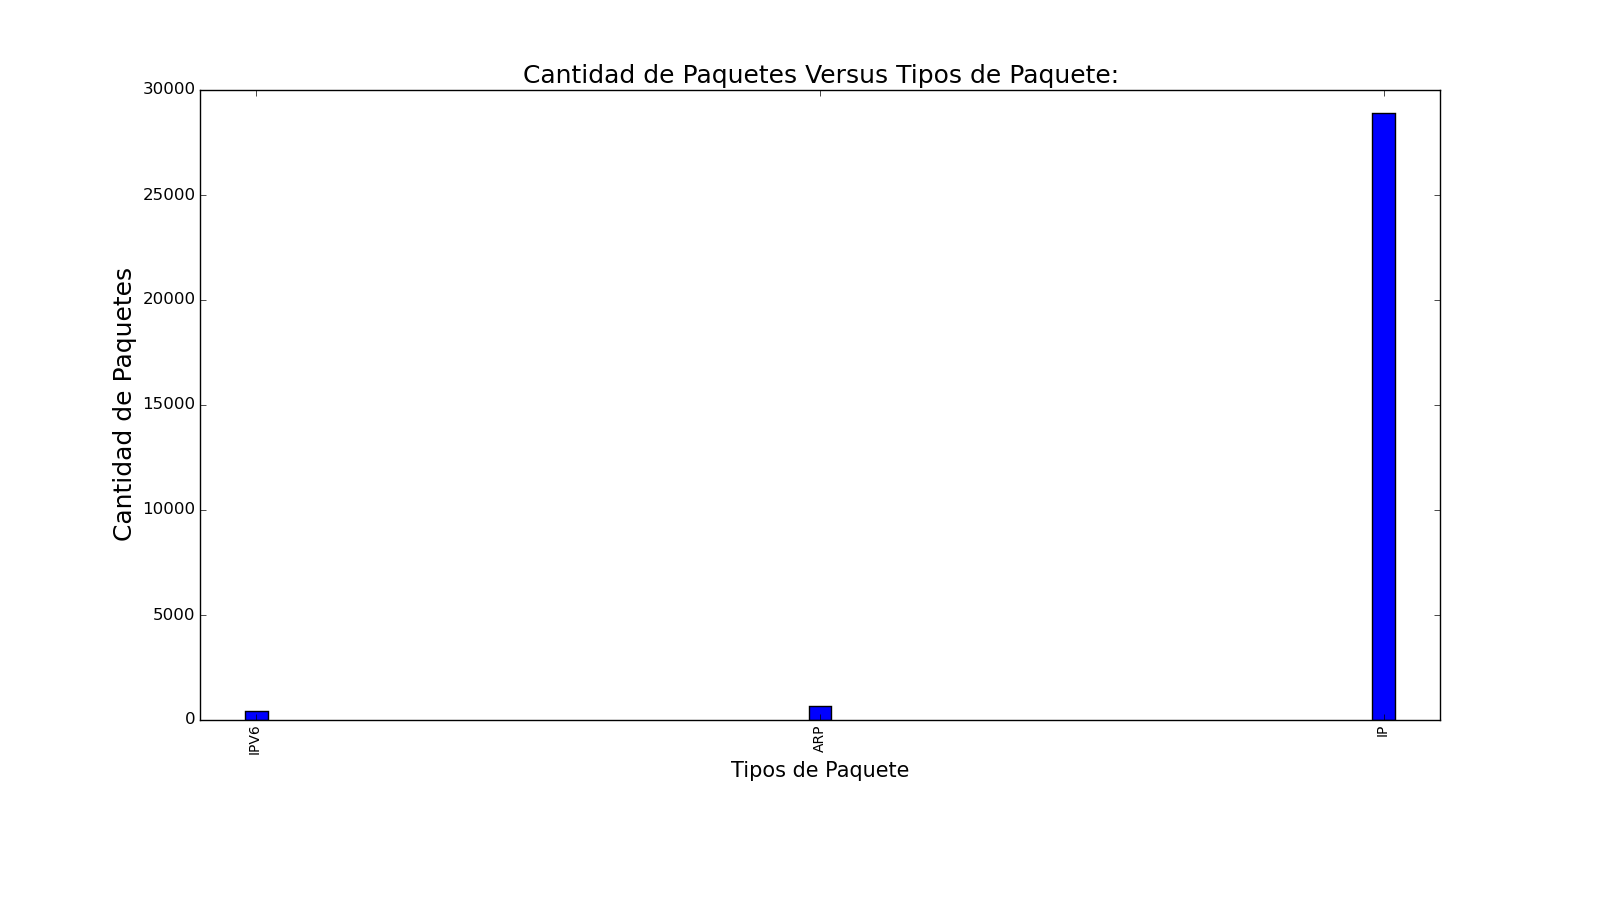
\includegraphics[width=1\textwidth]{../resultados/Starbucks/histogram_types.png}
       \caption{Protocolos de los paquetes capturados}
       \label{red-Starbucks-types}
\end{figure}

En este caso el overhead impuesto por los paquetes ARP es de 2.19\%

\begin{figure}[H]
       \centering
       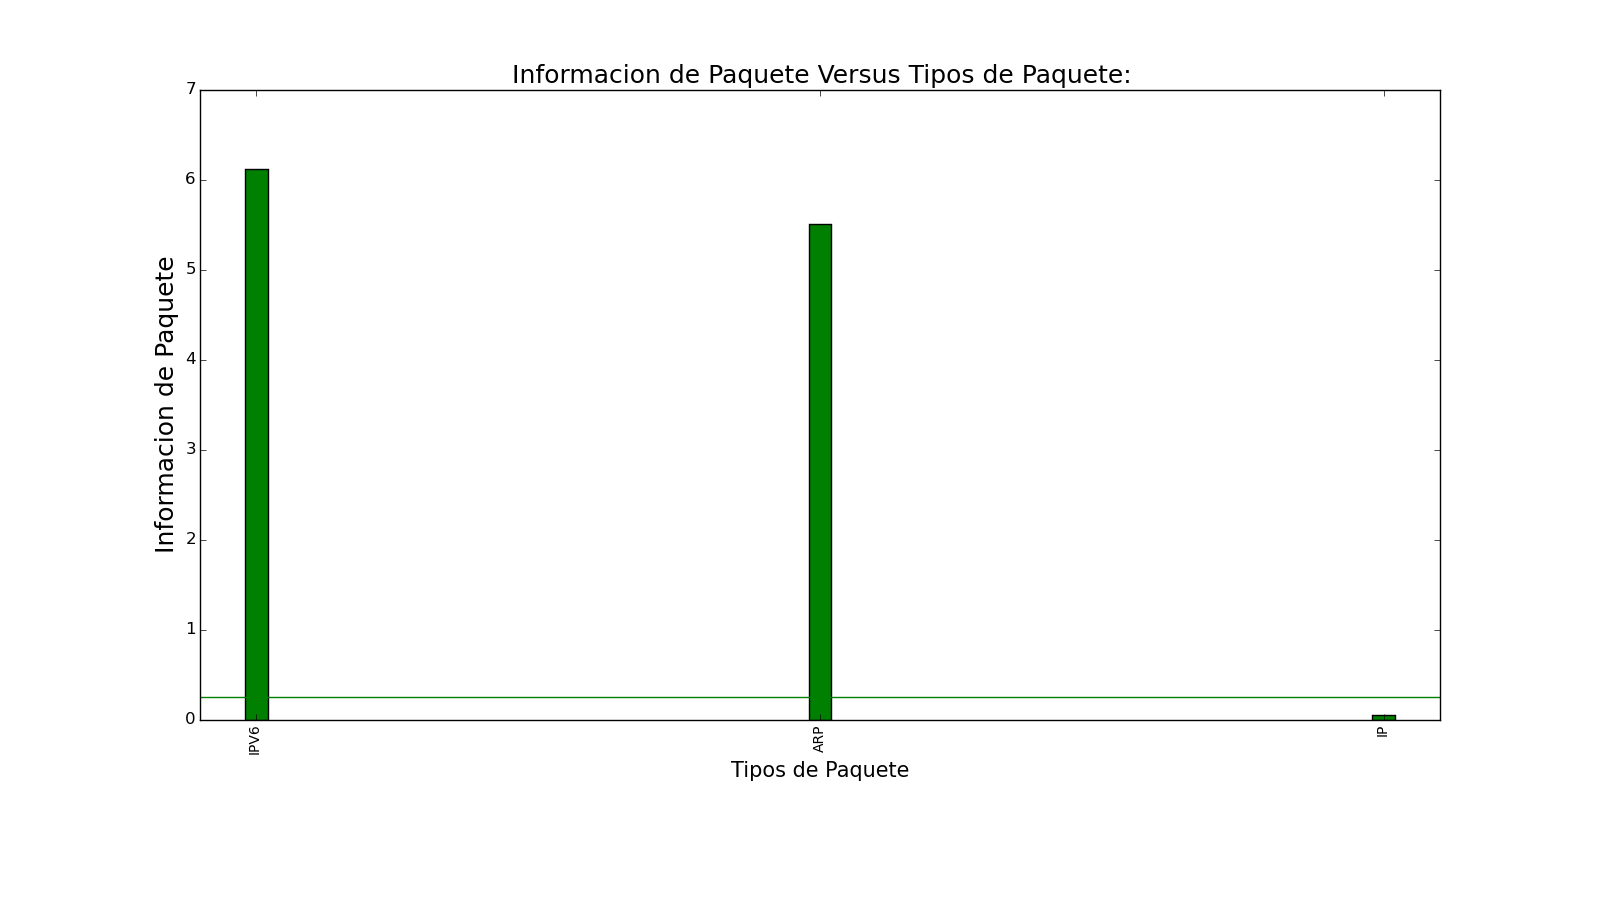
\includegraphics[width=1\textwidth]{../resultados/Starbucks/histogram_types_information.png}
       \caption{Información de los protocolos de los paquetes capturados}
       \label{red-Starbucks-types-information}
\end{figure}

Como podemos observar, de acuerdo a nuestra definición de protocolo distinguido, el protocolo IPv4 sería el único distinguido en esta fuente. Esto resulta razonable, ya que la cantidad de paquetes IPv4 es mucho mayor que la cantidad de paquetes IPv6 y ARP. La información de los paquetes IPv4 es \textbf{0.0532441907448}, mientras que la entropía de la fuente es \textbf{0.25983228318}. Se observa claramente como la información es menor a la entropía.

\begin{figure}[H]
       \centering
       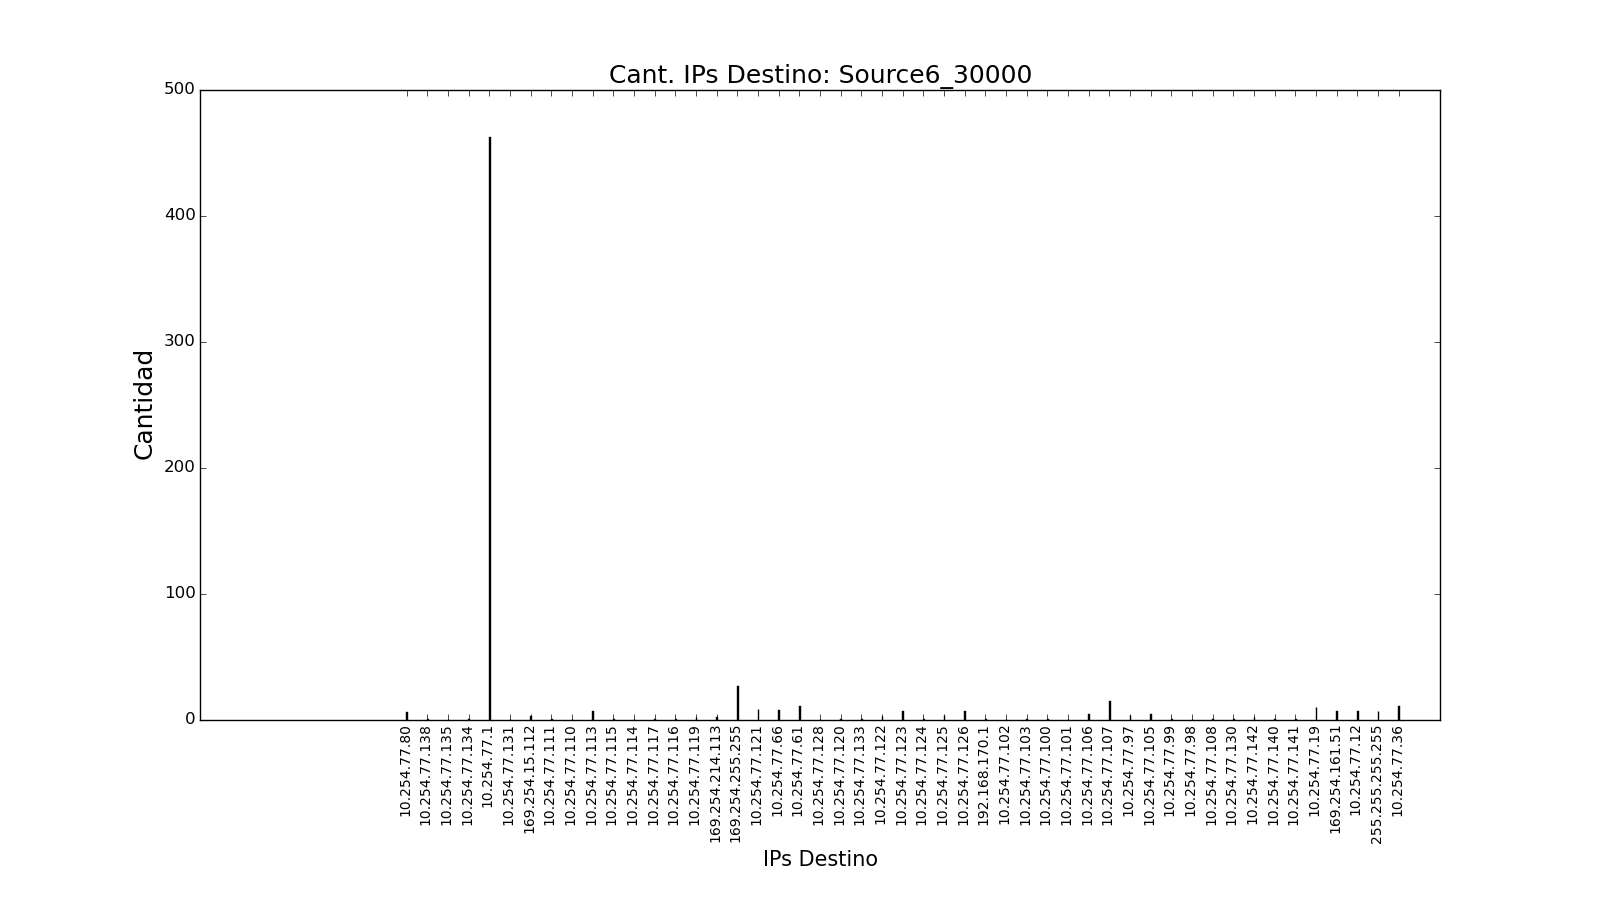
\includegraphics[width=1\textwidth]{../resultados/Starbucks/histogram_dst.png}
       \caption{IPs destino de los paquetes ARP}
       \label{red-Starbucks-dst}
\end{figure}


\begin{figure}[H]
       \centering
       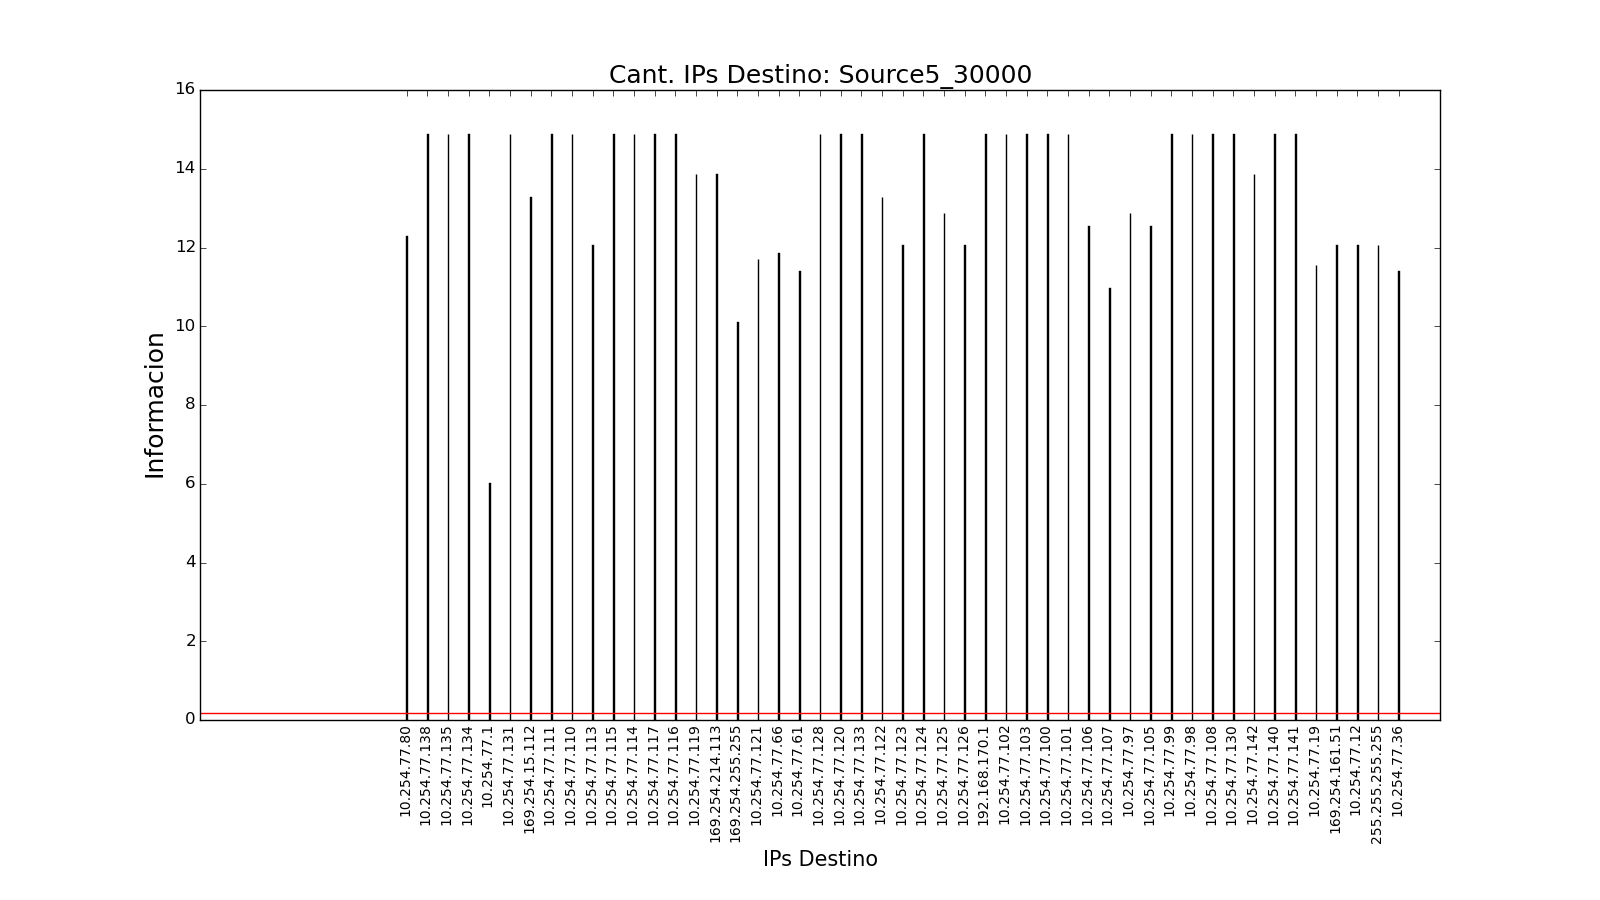
\includegraphics[width=1\textwidth]{../resultados/Starbucks/histogram_dst_information.png}
       \caption{Información de IPs destino de los paquetes ARP}
       \label{red-Starbucks-dst-information}
\end{figure}


\begin{figure}[H]
       \centering
       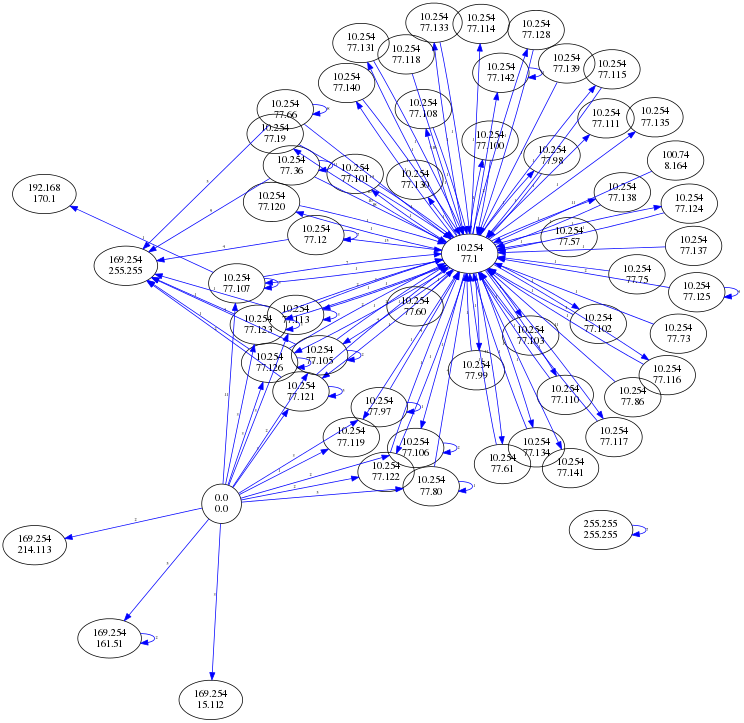
\includegraphics[width=1\textwidth]{../resultados/Starbucks/network.png}
       \caption{Tráfico de paquetes ARP}
       \label{red-Starbucks-dst-information}
\end{figure}

Apoyándonos en el hecho de que la IP \textbf{102.54.77.1} aparece con una gran ventaja respecto a las otras ip en cantidad, que además es un nodo distinguido por ser su información menor a la entropía y observando el gráfico de los nodos podemos concluir que es la IP del Router WiFi del local.

